Многие биологические объекты обладают периодической структурой. Например, зебра, дождевой червь, сороконожка. Однако известно, что изначально, при появлении, они однородны. Рассмотрим одномерный случай структур.

Тьюринг предположил, что существуют два вещества. Одно из них - $U(x,t)$ - стимулирует рост клеток. Его назвали активатором. Другое - $V(x,t)$ - замедляет рост. Это ингибитор. Следующим предположением было наличие некоторых химических реакций и присутствие диффузии. Фактически, Тьюринг записал уравнение реакции диффузии. 
\begin{equation}
\begin{cases}
		\pdv{U}{t}=f(U,V)+D_1 \pdv[2]{U}{x} \\
		\pdv{V}{t}=g(U,V)+D_2 \pdv[2]{V}{x},
	\end{cases}	\
	\label{eq:17}
\end{equation}
где $f,g$  - это некоторые нелинейные функции.

Эта система двухкомпонентная, произвольная координата одна. Предположим, \eqref{eq:17} имеет состояние равновесия, т.е. существует решение системы
\begin{equation}
\begin{cases}
		f(U,V)=0 \\
		g(U,V)=0.
	\end{cases}	\
	\label{eq:18}
\end{equation}
$U=U_0, V=V_0$.

Исследуем на устойчивость. Положим,
\begin{gather*}
	U=U_0+\xi(x,t) \\
	V=V_0+\eta(x,t).
\end{gather*}

Линеаризуем (оставляем только линейную часть):
\begin{equation}
	\begin{cases}
		\pdv{\xi}{t}=f'_u(U_0, V_0)\xi(x,t)+f'_v(U_0, V_0)\eta(x,t)+D_1 \pdv[2]{\xi(x,t)}{x} \\
		\pdv{\eta}{t}=g'_u(U_0, V_0)\xi(x,t)+g'_v(U_0, V_0)\eta(x,t)+D_2 \pdv[2]{\eta(x,t)}{x}.
	\end{cases}	
	\label{eq:19}
\end{equation}

Получили уравнения в частных производных. Будем искать решение в виде:
\begin{equation}
	\xi(x,t)=A e^{pt+ikx};~~\eta(x,t)=B e^{pt+ikx}.
	\label{eq:20}
\end{equation}

Подставляя эти решения и учитывая, что $f'$ и $g'$ - это производные в точке, т.е. константы, получим:
\begin{equation}
	\begin{cases}
		\pdv{\xi}{t}=a\xi+b\eta+D_1 \pdv[2]{\xi}{x} \\
		\pdv{\eta}{t}=c\xi+d\eta+D_2 \pdv[2]{\eta}{x},
	\end{cases}	
	\label{eq:21}
\end{equation}
где
\begin{gather*}
	a=f'_u(U_0, V_0),~~b=f'_v(U_0, V_0),~~c=g'_u(U_0, V_0),~~d=g'_v(U_0, V_0).
\end{gather*}

\begin{equation}
	\begin{cases}
		Ap=aA+bB-k^2 D_1A \\
		Bp=cA+dB-k^2 D_2A,
	\end{cases}	
	\label{eq:22}
\end{equation}

\eqref{eq:17} представляет собой систему линейных однородных уравнений относительно констант А,В. Она имеет нетривиальное решение, если ее определитель не равен нулю. Раскрывая определитель, получим характеристическое уравнение для p:
\begin{equation}
	p^2+(D_2k^2+D_1k^2-a-d)p+(D_1k^2-a)(D_2k^2-d)-bc=0.
	\label{eq:23}
\end{equation}

Предположим, что в начальный момент $D_1=D_2=0$, тогда
\begin{equation}
	p^2-(a+d)p+ad-bc=0.
	\label{eq:24}
\end{equation}

Сначала структуры у животных нет, следовательно, без диффузии имеем устойчивое равновесие. Запишем условие для этого:
\begin{gather*}
	\Delta_o=ad-bc>0, \\ \sigma_0=a+d<0,
\end{gather*}
тогда состояние равновесия будет устойчивым. 

\begin{figure}[H]
	\centering
	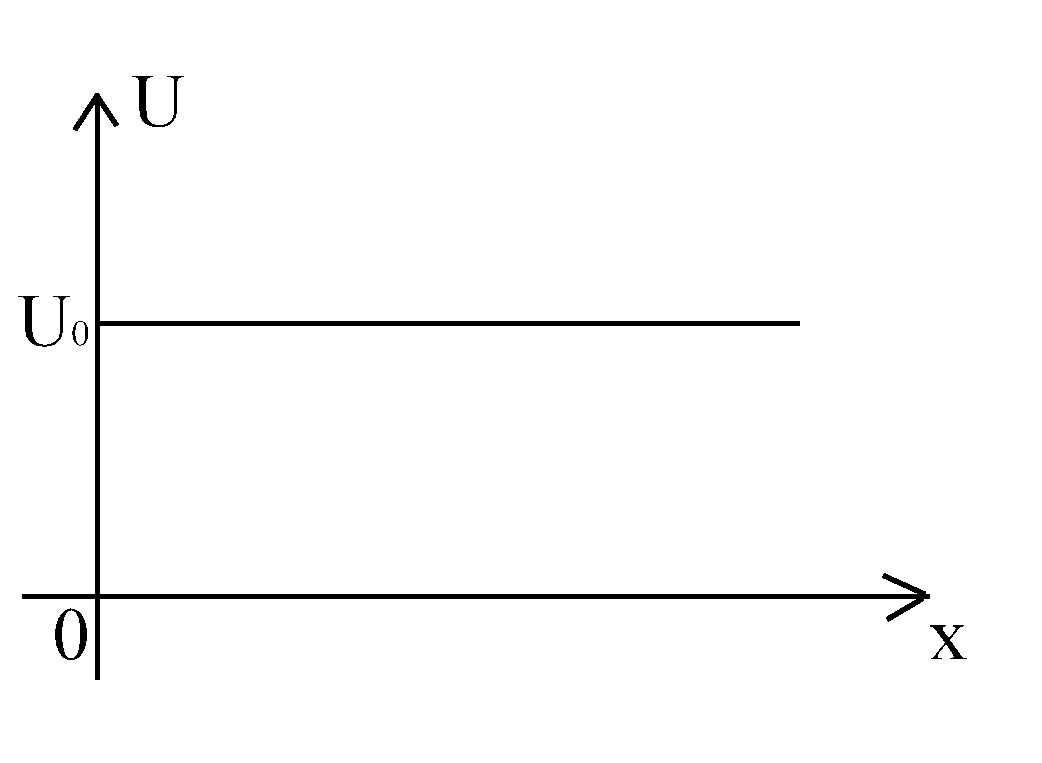
\includegraphics[width=0.5\linewidth]{fig/fig8.pdf}   
\end{figure}

По оси х U(активатор) и V(ингибитор) постоянны. 

Пусть теперь $D_1, D_2 \neq 0$. В этом случае \eqref{eq:24} после преобразований примет вид:
\begin{equation*}
	p^2-\sigma p+\Delta=0,
\end{equation*}
где
\begin{gather*}
	\Delta=a+d-(D_1+D_2)k^2=\sigma_0-(D_1+D_2)k^2, \\ \sigma=ad-bc-(aD_2+dD_1)k^2+D_1D_2k^4=\Delta_0-(aD_2+dD_1)k^2+D_1D_2k^4.
\end{gather*}

$Re\{p\}$ зависит от k. Анализ показывает:
\begin{figure}[H]
	\centering
	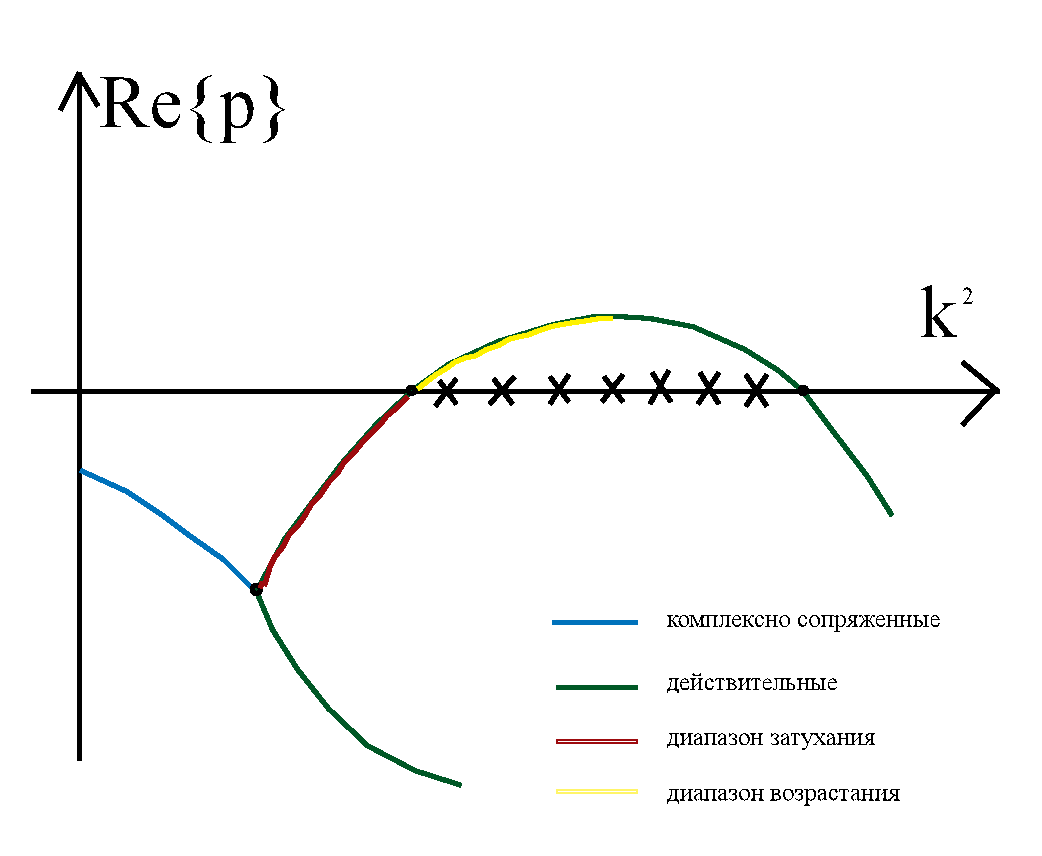
\includegraphics[width=0.5\linewidth]{fig/fig9.pdf}   
\end{figure}

Есть диапазон, где произошла потеря устойчивости состояния равновесия за счет действия диффузии. Это называется диффузионной неустойчивостью. Возникает аналог бифуркации Андронова-Хопфа. В диапазоне затухания все моды затухают, а возрастания - возрастают. Возникает периодическое по пространственной координате решение. Кроме того, оно пространственно неоднородное.  
\begin{figure}[H]
	\centering
	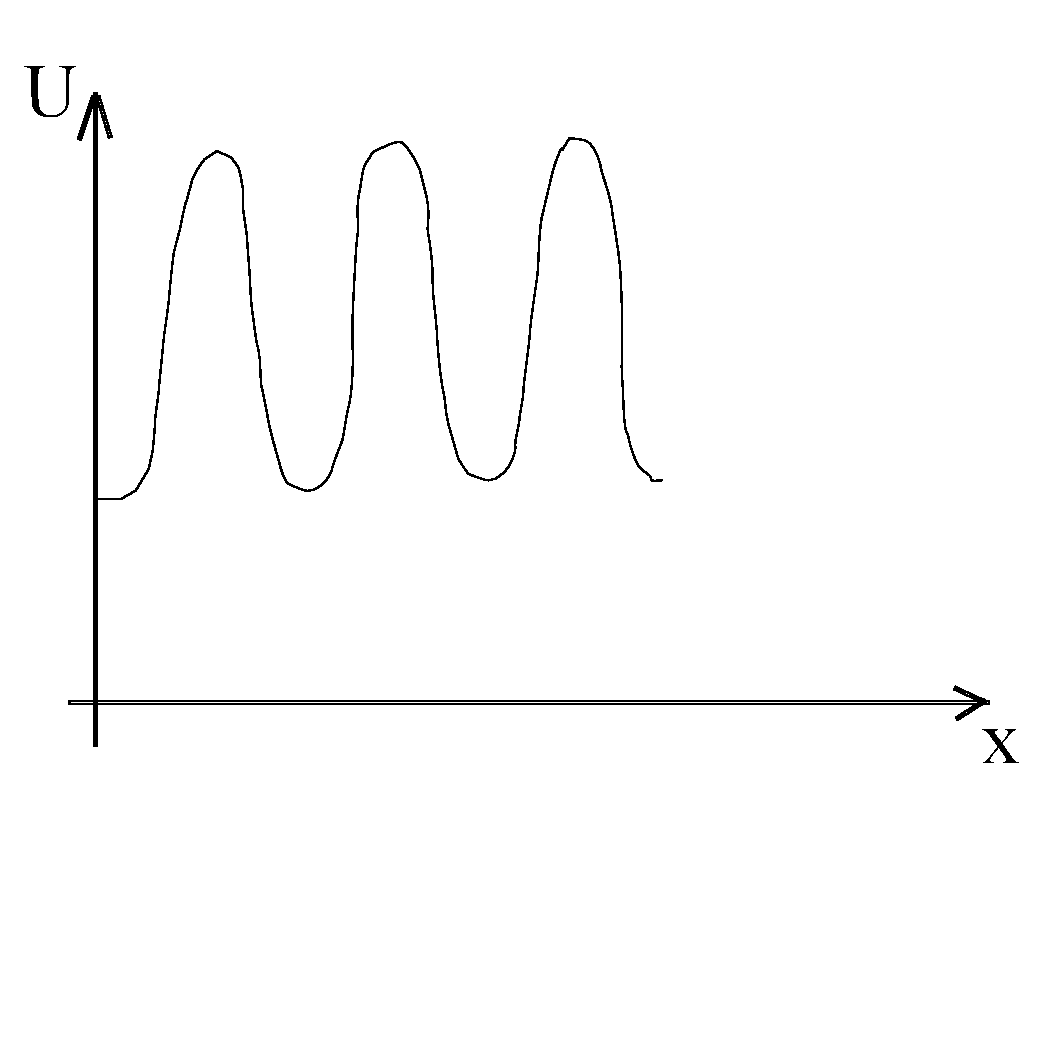
\includegraphics[width=0.5\linewidth]{fig/fig10.pdf}   
\end{figure}

Динамическая структура, обладающая свойством структурной устойчивости, иногда называется диссипативной структурой. Возникает за счет баланса. 

\subsection{Простые волны. Образование разрывов.}
Рассмотрим равномерную среду, свойства которой описывает скалярная функция $U(x,t)$. Среда линейная, без дисперсия. В таких средах возможно существование волновых движений, при этом все переменные описываются одинаковыми уравнениями:
\begin{equation}
	\pdv{U_j}{t}+V\pdv{U_j}{x}=0.
	\label{eq:25}
\end{equation}

В среде нет собственных масштабов и нелинейностей. V-const. В этой среде возможно существование так называемых римановых волн. 
\begin{equation}
	U_j=\phi(x-Vt),
	\label{eq:26}
\end{equation}
где $\phi$ - произвольная, обязательно дифференцируемая, функция.

Введем бегущую координату:
\begin{gather*}
	\xi=x-Vt, \\ \dv{\phi}{\xi} \pdv{\xi}{t}+V\dv{\phi}{\xi} \pdv{\xi}{x}=0, \\ -V\dv{\phi}{\xi}+V\dv{\phi}{\xi} \equiv 0.
\end{gather*}

\eqref{eq:26} является решением такой системы. 

Теперь рассмотрим нелинейную среду (но все еще без дисперсии). В таких средах могут существовать волны, которые обладают следующим свойством: переменные связаны алгебраически (если есть $U_1$ и $U_2$, то $U_3$ всегда можно пересчитать).

Рассмотрим пример: волны на мелкой воде. Гравитационные волны вдоль оси x.
\begin{figure}[H]
	\centering
	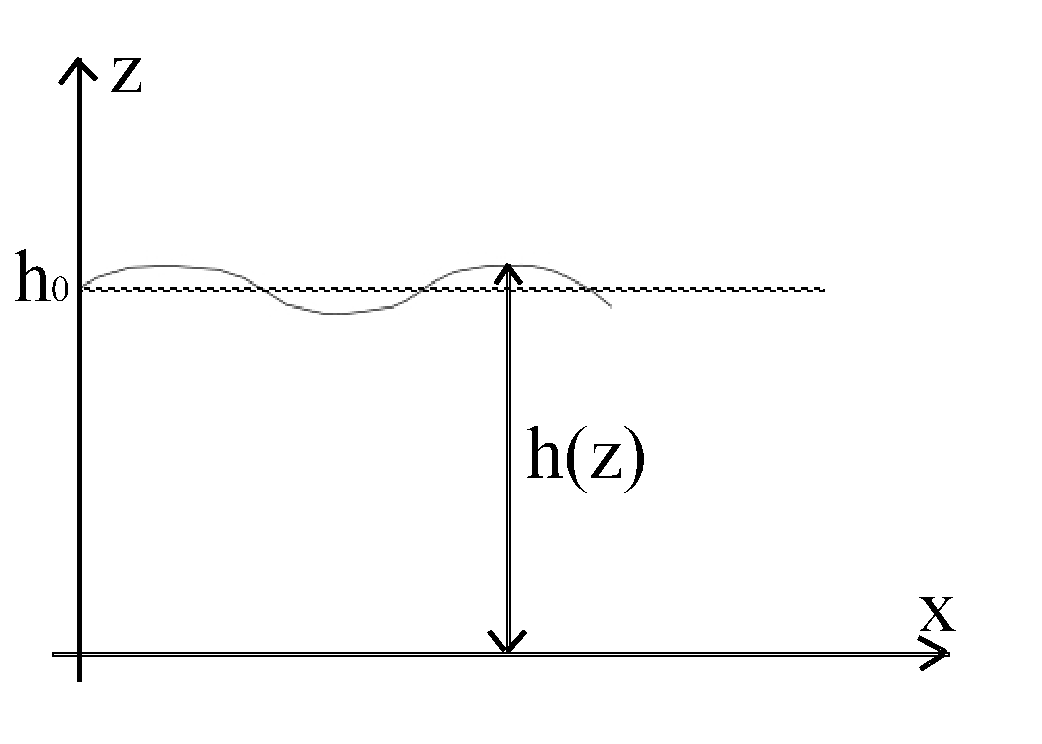
\includegraphics[width=0.4\linewidth]{fig/fig11.pdf}   
\end{figure}
$\lambda \gg h_0$

Состояние жидкости описывается: V - скоростью волны, h - профилем. Поскольку волны длинные, считаем, что $V\neq V(z)$.

Используем уравнение Эйлера: 
\begin{gather*}
	\pdv{V}{t}+V\pdv{V}{x}+\frac1{\rho}\pdv{\rho}{x}=0, \\ \rho=const, p-\text{среднее по высоте}, \\ \frac1{\rho}\pdv{\rho}{x}=g\pdv{h}{x}.
\end{gather*}

Давление больше там, где выше жидкость.
\begin{equation}
	\pdv{V}{t}+V\pdv{V}{x}+g\pdv{h}{x}=0.
	\label{eq:27}
\end{equation}

Добавим уравнение непрерывности:
\begin{gather*}
	\pdv{p}{t}+\pdv{(Vh)}{x}=0. 
\end{gather*}

Скорость изменения высоты слоя связана с разностью потока через x и dx
\begin{equation}
	\pdv{h}{t}+V\pdv{h}{x}+h\pdv{V}{x}=0.
	\label{eq:28}
\end{equation}

Предположим, h и V не являются независимыми переменными и $h=h(V)$.

Из уравнения \eqref{eq:27}: 
\begin{gather*}
	\pdv{h}{x}=\dv{h}{V}\pdv{V}{x}, \\ \pdv{V}{t}+V\pdv{V}{x}+g\pdv{h}{x} = 0 ~(*).
\end{gather*}

Из уравнения \eqref{eq:28}:
\begin{gather*}
	\dv{h}{V}\pdv{V}{t}+V\dv{h}{V}\pdv{V}{x}+h(V)\pdv{V}{x} = 0, \\ \pdv{V}{t}+V\pdv{V}{x}+\frac{h(V)}{\dv{h}{V}}\pdv{h}{x} = 0 ~(**).
\end{gather*}

(*) и (**) должны совпадать, т.к описывают одну и ту же величину. 
\begin{equation*}
	g\dv{h}{V}=\frac{h}{\dv{h}{V}}~ \text{или} ~(\dv{h}{V})^2=\frac{h}{g} - \text{уравнение для нахождения h}.
\end{equation*}

\begin{gather*}
	\dv{h}{V}=\pm \sqrt{\frac{h(V)}{g}}, \\ \pdv{V}{t}+V\pdv{V}{x}\pm \sqrt{h(V)g} \pdv{V}{x} = 0.
\end{gather*}
\begin{equation}
	\pdv{V}{t}+(V\pm \sqrt{h(V)g})\pdv{V}{x} = 0
	\label{eq:29}
\end{equation}
- уравнение простой волны, которое в общем виде выглядит:
\begin{equation}
	\pdv{U}{t}+V(U)\pdv{U}{x} = 0
	\label{eq:30}
\end{equation}

Это уравнение справедливо не только на мелкой воде. Здесь $V$ - это функция среды.

Будем искать решение в виде:
\begin{equation}
	U = \phi(x-V(U)t),
	\label{eq:31}
\end{equation}
\begin{gather*}
	\xi=x-V(U)t.
\end{gather*}

Убедимся, что \eqref{eq:30} - решение:
\begin{gather*}
	\pdv{U}{t}=\dv{\phi}{\xi}\pdv{\xi}{t}=\dv{\phi}{\xi}\qty(-V(U)-t\dv{V}{U}\pdv{U}{t}), \\ \pdv{U}{t}\qty(1+\dv{\phi}{\xi}\dv{V}{U}t)=-V(U)\dv{\phi}{\xi},
\end{gather*}
\begin{equation}
	\pdv{U}{t}=-V(U)\dv{\phi}{\xi} \frac{1}{(1+\dv{\phi}{\xi}\dv{V}{U}t)}
	\label{eq:32}
\end{equation}
\begin{gather*}
	\pdv{U}{x}=\dv{\phi}{\xi} \frac{1}{(1+\dv{\phi}{\xi}\dv{V}{U}t)}
\end{gather*}

Для определенности:
\begin{figure}[H]
	\centering
	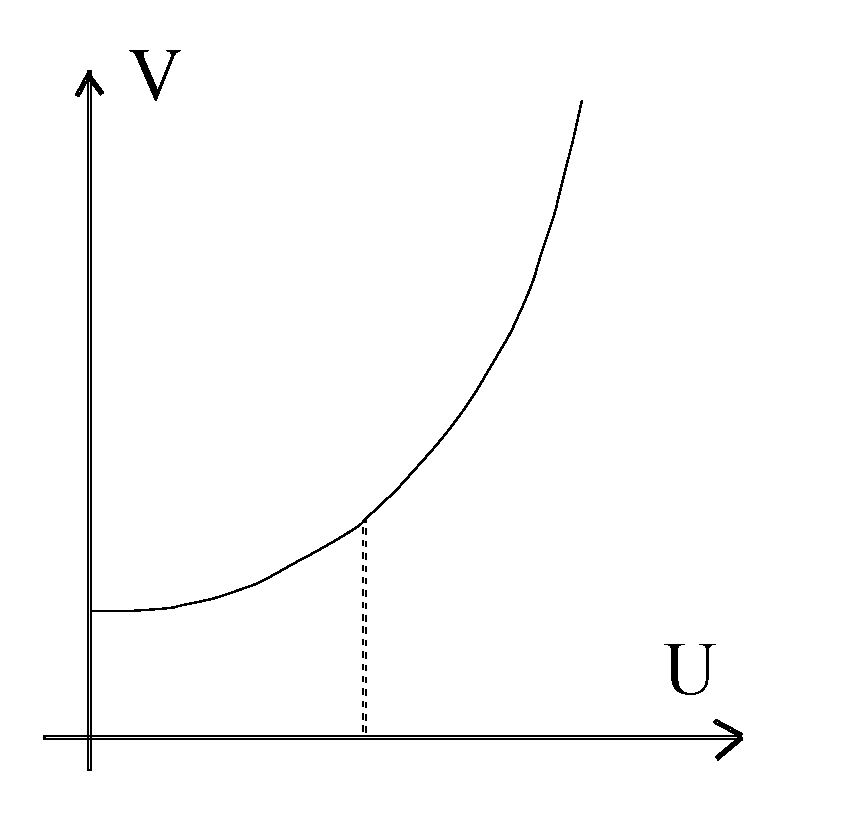
\includegraphics[width=0.4\linewidth]{fig/fig12.pdf}   
\end{figure}

У максимального значения U скорость наибольшая. Задается профиль $\phi$ при $t=0$:
\begin{figure}[H]
	\centering
	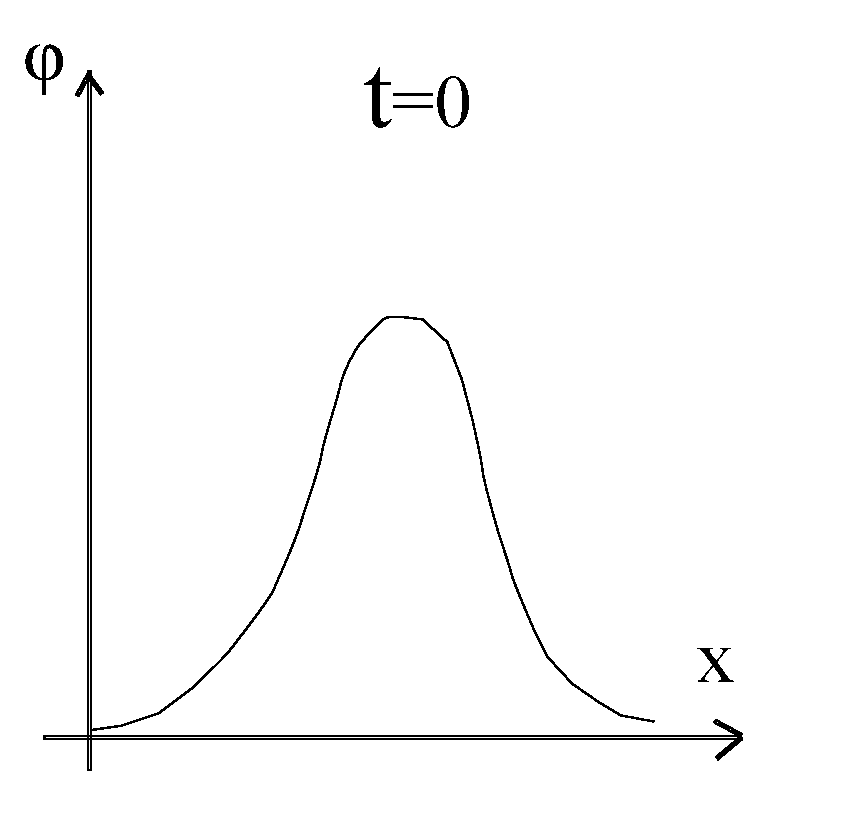
\includegraphics[width=0.4\linewidth]{fig/fig13.pdf}   
\end{figure}
или при $x=0$:
\begin{figure}[H]
	\centering
	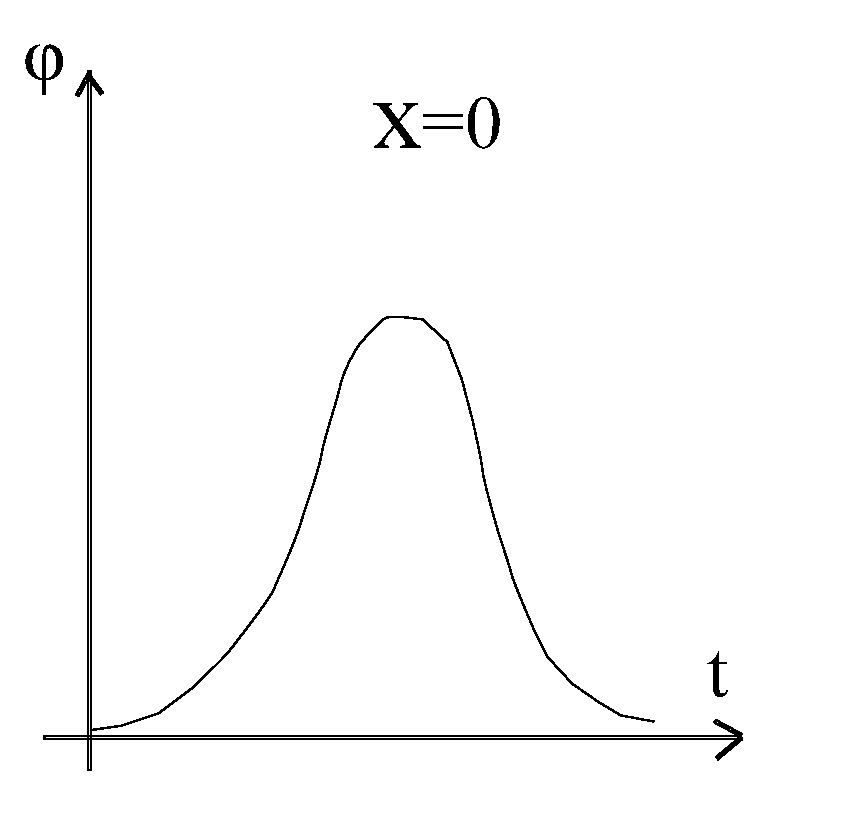
\includegraphics[width=0.4\linewidth]{fig/fig14.pdf}   
\end{figure}

Во время распространения, верх волны обгонит, произойдет укручение фронта, волна деформируется. 
\begin{figure}[H]
	\centering
	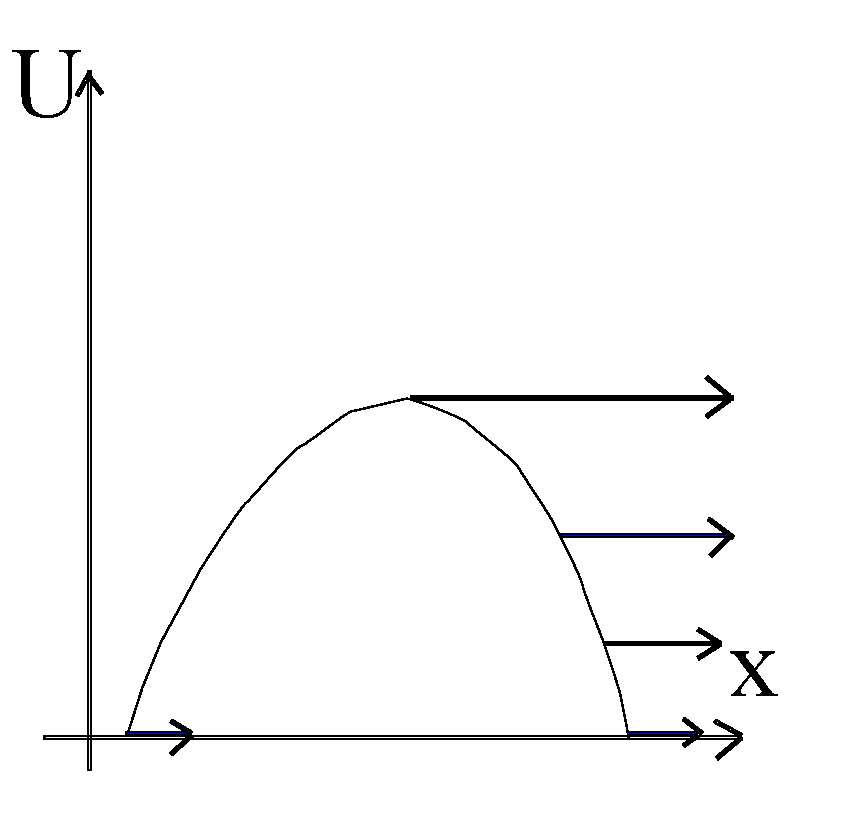
\includegraphics[width=0.4\linewidth]{fig/fig15.pdf}   
\end{figure}
\begin{figure}[H]
	\centering
	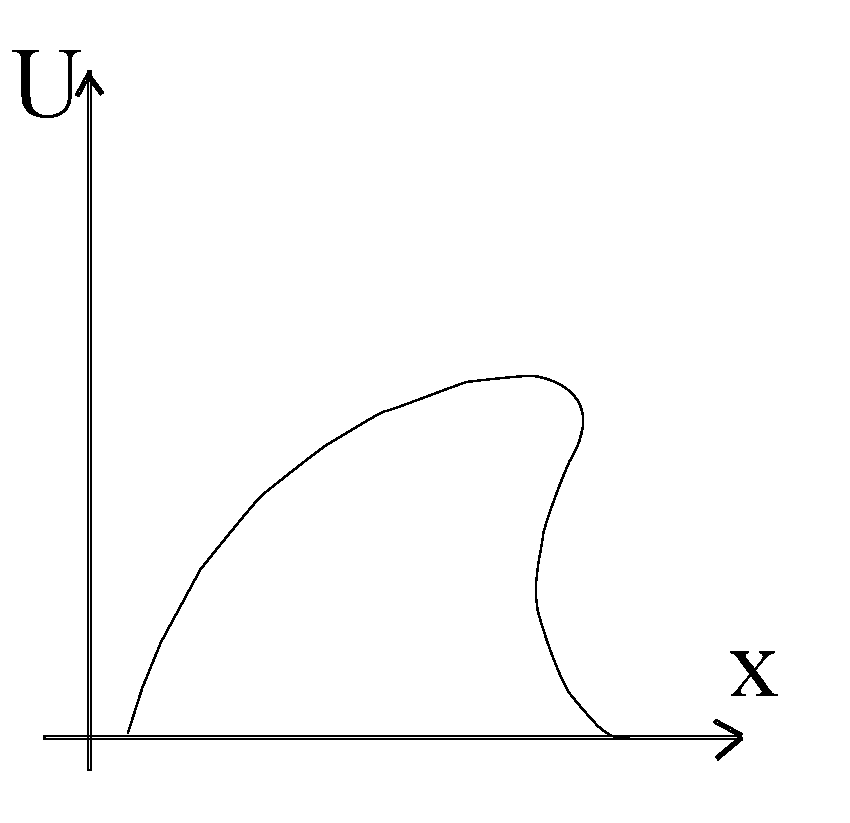
\includegraphics[width=0.4\linewidth]{fig/fig16.pdf}   
\end{figure}
\begin{figure}[H]
	\centering
	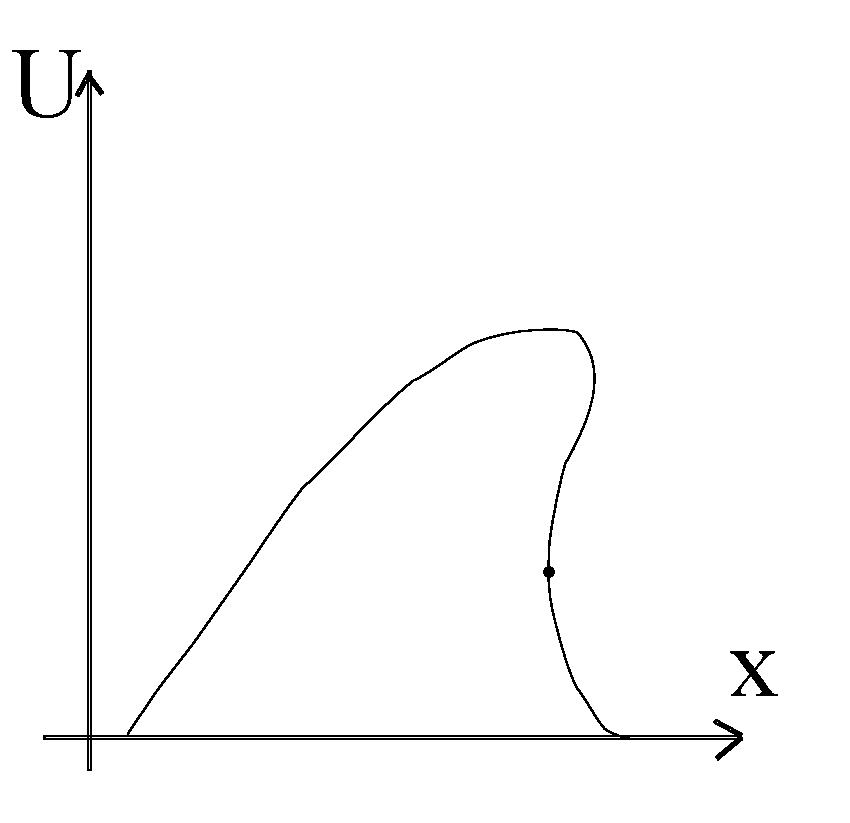
\includegraphics[width=0.4\linewidth]{fig/fig17.pdf}   
\end{figure}

Появится точка, где производные $\pdv{U}{t}, \pdv{U}{x} \rightarrow \infty $. Образуется бесконечный градиент и разрыв, который характеризуется состоянием $U^*, t^*, x^*$, его описание в рамках простой волны несправедливо. Вторые производные тоже обращаются в бесконечность, и точки эти можно найти.